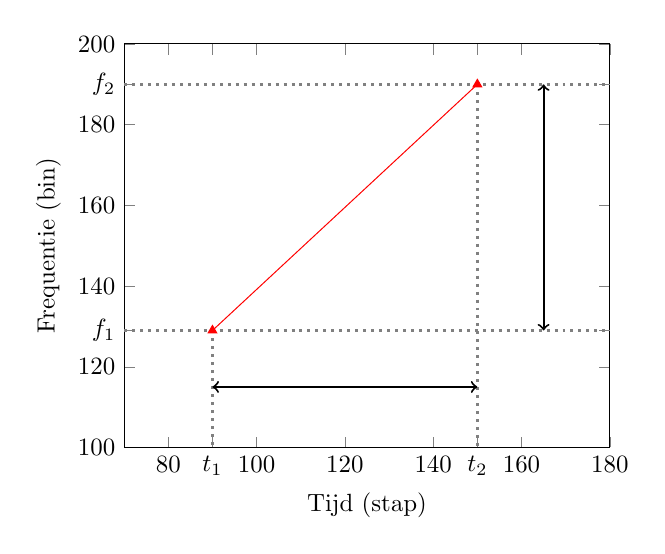
\begin{tikzpicture}[scale=0.9]
\begin{axis}[
	xlabel={Tijd (stap)},
	ylabel={Frequentie (bin)},
	xmin=70,xmax=180,
	ymin=100,ymax=200,
	legend style={
  		cells={anchor=west},
  		legend pos=outer north east,
	},
	extra y ticks={129,190}, 
	extra y tick labels={$f_1$,$f_2$},
	extra x ticks={90,150}, 
	extra x tick labels={$t_1$,$t_2$},
]

  % plot the data from the file data.dat
  % smooth the curve and mark the data point with a dot
  \addplot[color=red,mark=triangle*] coordinates {
  	(90,129)
  	(150,190)
  };
  
  %f1
   \addplot[style= dotted,color=gray,very thick] coordinates{ (70,129)
   (180,129)};
   %f2
   \addplot[style= dotted,color=gray,very thick] coordinates{ (70,190)
   (180,190)};
   
    \node at (99,60) [] {\small$\Delta f$};
    \addplot[color=black,<->,thick] coordinates{ (165,129) (165,190)};
    
   \node at (50,18) [] {\small$\Delta t$};
   \addplot[style=dotted,color=gray,very thick] coordinates{ (90,129)
   (90,100)}; 
   \addplot[style=dotted,color=gray,very thick] coordinates{
   (150,190) (150,100)};
   \addplot[color=black,<->,thick] coordinates{ (90,115)
   (150,115)};
  
  \end{axis}
\end{tikzpicture}